% !TeX root = ../main.tex

\section*{Markov Random Fields (MRF)}

\paragraph{Idea:} An image $G$, given by the random matrix $[g_{i,j}]$ can be considered as a pixel grid of random variables.

%Example use cases are denoising, segmentation or stereo matching. 

\begin{equation*}
    p([g_{i, j}]) = \prod_{i,j} p(g_{i, j} | g_{i-1, j} g_{i, j-1} g_{i-1, j-1})
\end{equation*}

\paragraph{Definition of MRF:}
\begin{enumerate}
    \item Positivity:\footnote{For a certain observation the probability is non zero} $ p(\vec{x}_1, \vec{x}_2, \dots, \vec{x}_N) > 0$
    \item Markov property:\footnote{where $\mathcal{N}(\vec{x}_k))$ denotes the neighborhood of $\vec{x}_k$: 1. $\vec{x}_k \notin \mathcal{N}(\vec{x}_k)$; 2. $\vec{x}_i \in \mathcal{N}(\vec{x}_k) \Leftrightarrow \vec{x}_k \in \mathcal{N}(\vec{x}_i)$: 3. $\mathcal{N}(\vec{x}_k) = \{x_i|0 < dist(x_i, x_k) \le t\}$} $ p(\vec{x}_k |\vec{x}_1, \dots, \vec{x}_{k-1}, \vec{x}_{k+1}, \dots, \vec{x}_N) = p(\vec{x}_k | \mathcal{N}(\vec{x}_k)) $
\end{enumerate}


\begin{figure}[H]
  \centering
  \begin{minipage}[b]{0.45\textwidth}
    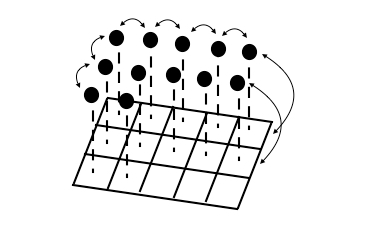
\includegraphics[width=\textwidth]{mrf_image_example}
		\caption{The idea of MRF on images the arrows indicate relations}
  \end{minipage}
  \begin{minipage}[b]{0.45\textwidth}
    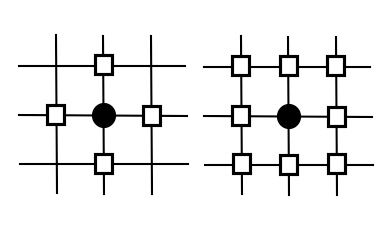
\includegraphics[width=\textwidth]{mrf_grid_neighborhood}
		\caption{4-Neighborhood, 8-Neighborhood (and dynamic-Neighborhood)}
  \end{minipage}
\end{figure}

Two criteria for the hidden variables: Neighbors should be similar to each other; a hidden variable should still resemble the original observation (random variable).
The neighborhoods can also be decomposed in graph Cliques (complete subgraphs) of two. Which is useful later on (factorization + there are solvers for two variables)

\paragraph{Gibbs Random Fields (GRF):} is given by the PDF

\begin{equation*}
	p(x) = \frac{1}{Z} e^{-H(x)}
\end{equation*}

where $Z = \sum_{x^\prime} H(x^{\prime})$ is a partition function and $H(x)$ an energy function, i.e. a sum of potential functions.

\paragraph{Remark:}
For a given PDF $p(x)$, the choice of the energy function $H(x)$ is not unique. Consider for example

\begin{equation*}
	H(x) = - \log p(x) - \log Z
\end{equation*}

\begin{equation*}
	p(x) = \frac{1}{Z} e^{-H(x)} = \frac{1}{Z} e^{\log p(x)} e^{\log Z}  = p(x)
\end{equation*}

$\rightarrow$ we can choose $Z$ arbitarily\\

\paragraph{Hammersley-Clifford Theorem:} proves that GRFs and MRFs are equivalent. This means we can model the neighborhood relationships in our MRF in terms the energy and potential functions of the GRF.

\paragraph{Example:} Image denoising

Given: The observed noisy image $[g_{i,j}]$

Searched: Hidden variables are the ideal (noiseless) image $[f_{i,j}]$\\

\textbf{MRF criterium 1:} The ideal image is spatially smooth

\begin{equation*}
	p(f_{i,j}]) = \frac{1}{Z} e^{-H([f_{i,j}])}, \quad \text{where } H([f_{i,j}]) = \sum_{i,j} ||\nabla f_{i,j}||_2^2 \qquad (||\nabla f_{i,j}||_2^2 \text{ function of clique of size 2})
\end{equation*}
$ H([f_{i,j}]) $ is sum of squared gradients, computed over a neighborhood (or the sum over all clique potentials).\\

\textbf{MRF criterium 2:} $[g_{i,j}]$ is similar to $[f_{i,j}]$, but corrupted by additive Gaussian noise

\begin{equation*}
	p([g_{i,j}] | f_{i,j}]) = \prod_{i,j} \frac{1}{\sqrt{2 \pi} \sigma_{i,j}} \exp\Big(- \frac{1}{2 \sigma_{i,j}^2} \cdot \underset{\text{energy function $H$}}{(f_{i,j} - g_{i,j})^2}\Big)
\end{equation*}

With these two functions defined, we can solve for a MAP estimate for $f$:

\begin{align*}
	\underset{\text{estimated ideal image}}{[\hat{f}_{i,j}]} &= \argmax_{[f_{i,j}]} p([f_{i,j}] | [g_{i,j}])\\
					&= \argmax_{[f_{i,j}]} \big(p([f_{i,j}] \cdot p([g_{i,j}] | [f_{i,j}])\big)\\
					& \dots\\
					&= \argmin_{[f_{i,j}]} \Big(\sum_{i,j} ||\nabla f_{i,j}||_2^2 + \sum_{i,j} \lambda_{i,j} (f_{i,j} - g_{i,j})^2\Big)
\end{align*}

% TODO: Max Flow / Min Cuts
